\RequirePackage[T1]{fontenc}
\documentclass[conference]{IEEEtran}
\usepackage{times}
\usepackage[numbers]{natbib}
\usepackage{graphicx}
\usepackage{capt-of}
\usepackage{caption}
\usepackage{booktabs}
\usepackage{array}
\usepackage{tabularx}
\usepackage{amsmath,amssymb}
\usepackage{xcolor}
\usepackage{microtype}
\usepackage[section]{placeins}
\usepackage[hidelinks,breaklinks=true,bookmarks=false]{hyperref}
% Verified Anonymous GitHub website; expires on 2027-09-11.
\newcommand{\projectpageurl}{https://anonymous.4open.science/w/ForceDelta-VLA/}
\newcommand{\projectpagestatement}{%
    \ifx\projectpageurl\empty\else
    Project page:~{\color{magenta}\expandafter\nolinkurl\expandafter{\projectpageurl}}.%
    \fi
}



% comments
% \newcommand{\lzhang}[1]{\textcolor{magenta}{#1}}
\newcommand{\lzhang}[1]{\textcolor{black}{#1}}

\IEEEoverridecommandlockouts                              % This command is only needed if
                                                          % you want to use the \thanks command

\title{\LARGE\bfseries
ForceDelta-VLA: Distilling Force-Conditioned Action\\Corrections for Contact-Rich Manipulation}

\newcommand{\isanonymous}{}  % Double-blind review mode
% IEEE not suppoer Minted，use lstlisting during submission

% \author{Anonymous CVPR submission \\ Paper ID 000}
\ifdefined\isanonymous
    \author{Anonymous Authors}
\else
    \author{
        Ju Dong$^{1}$,
        Yimeng Liu$^{2}$,
        Jian Chen$^{3}$,
        Yu Fu$^{1}$, 
        Haocheng Zhao$^{2}$,\\
        Kaixin Bai$^{1}$,
        Liding Zhang$^{2}$,
        %Zhaopeng Chen$^{2}$,
        Lei Zhang$^{1\dag}$,
        Alois Christian Knoll$^{2}$,
        Jianwei Zhang$^{1}$ % <-this % stops a space
        % \thanks{\dag The first two authors contribute equally to this paper.}
        \thanks{\dag Corresponding author. lei.zhang-1@studium.uni-hamburg.de}
        \thanks{* The authors contributed equally to this work.}
        \thanks{$^{1}$TAMS (Technical Aspects of Multimodal Systems), Department of Informatics, University of Hamburg, Hamburg, Germany. 
        }
        %\thanks{$^{2}$Agile Robots SE, Munich, Germany.
        % ~\texttt{\{name.surname\}@agile-robots.com}
        %}
        \thanks{$^{2}$Technical University of Munich, Germany. 
        % \texttt{\{name.surname\}@tum.de}
        }
        \thanks{$^{3}$University of Science and Technology of China, Hefei, China.
        }
    }
\fi

\begin{document}
    \makeatletter
    \let\@oldmaketitle\@maketitle
    \renewcommand{\@maketitle}{\@oldmaketitle
      \centering
      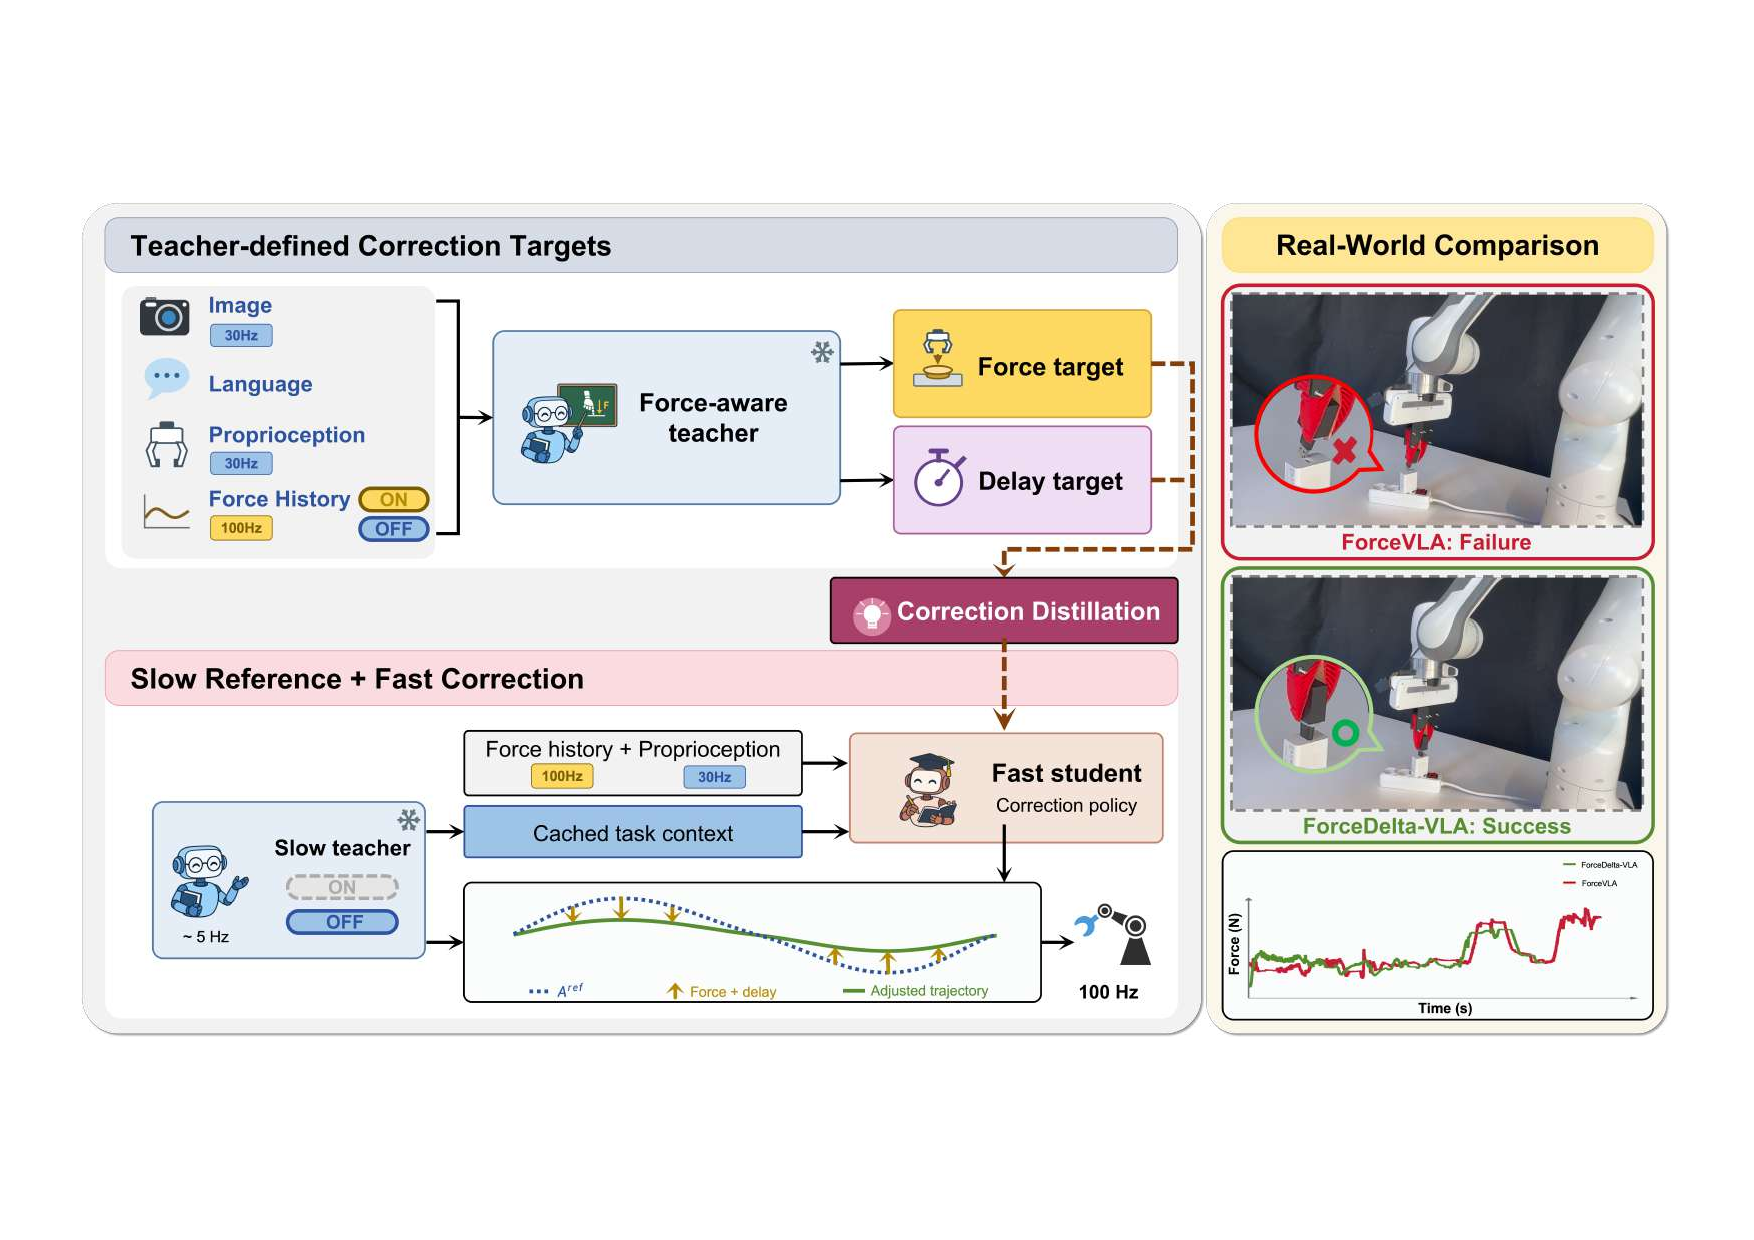
\includegraphics[width=\textwidth]{figures/fig01_method_overview.pdf}
      % \vspace{-0.2in}
      \captionof{figure}{ForceDelta-VLA overview. A frozen teacher provides force and delay correction targets to train a lightweight student. During execution, the student jointly predicts both corrections to adjust reference actions from the slow teacher.}
      \label{fig:teaser}
      \vspace{-0.1in}
      \bigskip}
\makeatother
\maketitle

\thispagestyle{empty}
\pagestyle{empty}
\setcounter{figure}{1}
\begin{abstract}
Force-aware Vision-Language-Action (VLA) policies improve contact-rich manipulation, but typically combine task-level motion and contact-dependent adjustment in a single action prediction. Demonstrations provide no explicit labels for decomposing that prediction into a reusable reference action and a correction. We present ForceDelta-VLA, a correction-distillation framework that constructs an explicit force-correction target from paired force-conditioned and learned force-agnostic predictions of a frozen teacher. A separate delay-correction target accounts for reference-action mismatch and the change in reference state. Training uses asynchronous schedule replay with the cached task context available during execution. The resulting lightweight policy adjusts the reference actions using recent force history and robot state, responding to contact changes between reference-action updates without regenerating complete action chunks. Across nine single-arm and bimanual contact-rich tasks, ForceDelta-VLA achieves an $82.2\%$ mean success rate, compared with $54.4\%$ for the original ForceVLA baseline. Our Stage-1 Temporal Teacher uses the same temporal force-aware backbone and achieves $70.6\%$ under direct execution. Relative to ForceVLA, the complete system reduces mean successful-trial peak contact force by approximately $26\%$ on both platforms.
\projectpagestatement
\end{abstract}

\section{Introduction}
Contact-rich manipulation requires actions to adapt as contact develops. During USB insertion, for example, the approach direction may remain useful over nearby control cycles, while local alignment must respond to newly observed contact. Force-aware Vision-Language-Action (VLA) policies incorporate interaction feedback into action generation~\cite{yu2025forcevlaenhancingvlamodels,li2026forcevla2unleashinghybridforceposition,zhang2025tavlaelucidatingdesignspace}, but typically predict task motion and contact-dependent adjustment together. Separating a reference action predicted by a slow pathway from a rapidly updated correction would allow contact feedback to affect execution without waiting for a new complete action chunk (Fig.~\ref{fig:teaser}).

Learning this correction from offline demonstrations is not straightforward. Demonstrations record the final action, without specifying which part belongs to the base behavior and which part is a contact-dependent adjustment. Multiple additive decompositions can reconstruct the same label. A correction pathway therefore needs a defined supervision target in addition to a fast architecture.

Existing asynchronous policies separate computation or sensor-update rates~\cite{li2026favlaforceadaptivefastslowvla,wang2026lateforceacceleratingvla,vanjani2026damvladecoupledasynchronousmultimodal}. Residual reinforcement learning and corrective imitation obtain correction signals from rewards or extra on-policy interaction~\cite{ankile2024imitationrefinementresidual,xu2025compliantresidualdaggerimproving}. We address the supervision problem using only the original offline demonstration dataset, while retaining asynchronous execution.

We present ForceDelta-VLA, which uses a lightweight policy to update force and delay corrections independently of reference-action generation. In offline training, paired force-conditioned and learned force-agnostic predictions of a frozen teacher define the force-correction target. The paired queries share task context, robot state, and sampling noise. A separate delay-correction target compensates for the mismatch between the previous reference action and the current force-agnostic prediction, including their different state references. Asynchronous schedule replay constructs these targets using the cached context available at deployment. During execution, the lightweight policy adjusts reference actions from the slow pathway using recent observations, responding to changes in robot state and contact between reference-action updates. The paired teacher queries are used only to construct training targets.

We evaluate ForceDelta-VLA on five single-arm and four bimanual real-robot tasks spanning contact establishment, precision insertion, friction-dominated motion, and constrained manipulation. The method achieves an $82.2\%$ mean success rate, compared with $54.4\%$ for ForceVLA and $70.6\%$ for direct rollout of the Temporal Teacher. Relative to ForceVLA, it reduces mean successful-trial peak contact force by approximately $26\%$ on both platforms. The correction forward pass takes $2.43$~ms.

The contributions of this work are:
\begin{enumerate}
    \item We introduce \textbf{force-agnostic correction distillation}: an explicit teacher-defined force-correction target from matched force-conditioned and learned force-agnostic predictions of a frozen teacher, using only the original offline dataset;
    \item We formulate a \textbf{state-consistent dual-correction decomposition} that separately supervises force and delay corrections in a common action coordinate system, with the delay target incorporating both reference-action mismatch and state rebasing; and
    \item We develop an \textbf{independently executable correction pathway} that updates pose corrections from recent force history and robot state while reusing reference actions and task context from the slow pathway.
\end{enumerate}


\section{Related Work}
\label{sec:related}
\subsection{Force-Aware Manipulation Policies}
Force-aware policies incorporate interaction feedback into action prediction~\cite{yu2025forcevlaenhancingvlamodels,li2026forcevla2unleashinghybridforceposition,zhang2025tavlaelucidatingdesignspace,li2026fmvlaforcebasedmemoryvisionlanguageaction,zhang2026craftadaptingvlamodels,liu2025forcemimicforcecentricimitationlearning}. These methods typically predict task motion and contact adjustment together. ForceDelta-VLA separates a reusable reference action from corrections driven by recent wrench feedback. This also differs from FD-VLA, which distills a force representation for inference without measured wrench feedback~\cite{zhao2026fdvlaforcedistilledvisionlanguageactionmodel}.

\subsection{Multi-Rate and Structured Manipulation Policies}
Prior policies separate sensing, action generation, and correction across different update rates~\cite{lee2025manipforceforceguidedpolicylearning,chen2026implicitrdpendtoendvisualforcediffusion,wang2026phaforcephasescheduledvisualforcepolicy,fang2026forcepolicylearninghybrid,zhuo2026fardp}. FAVLA and DAM-VLA extend multi-rate processing to VLAs~\cite{li2026favlaforceadaptivefastslowvla,vanjani2026damvladecoupledasynchronousmultimodal}, while RTC addresses continuity between asynchronously generated action chunks~\cite{black2025realtimechunking}. Our focus is on updating teacher-defined force and delay corrections while reusing a reference action, independently of complete action generation.

\subsection{Residual Policy Learning}
Residual policies add learned corrections to a base controller~\cite{johannink2018residualreinforcementlearningrobot}. Prior methods learn these corrections from rewards or on-policy human corrections~\cite{ankile2024imitationrefinementresidual,xu2025compliantresidualdaggerimproving,yu2026omnitactunepolicyagnosticrealworldrl,wang2026lateforceacceleratingvla}, or impose an additive structure during imitation learning~\cite{wang2026phaforcephasescheduledvisualforcepolicy}. ForceDelta-VLA instead constructs explicit correction targets from paired teacher predictions using the original demonstration dataset.

\subsection{Policy Distillation}
Robot-policy distillation often accelerates full-action generation~\cite{wang2024onestepdiffusionpolicyfast,dong2026flowsteprealtimemultimodal}. ForceDelta-VLA distills corrections and retains the generative teacher for reference actions. Its paired targets build on the idea of transferring conditional updates through guidance distillation~\cite{ho2022classifierfreediffusionguidance,meng2023distillationguideddiffusionmodels}. The learned force-agnostic mode distinguishes unavailable force input from measured zero force, following missing-modality learning~\cite{ramazanova2024exploringmissingmodalitymultimodal,nezakati2024mmprobustmultimodallearning}.


\section{Method}\label{sec:method}

\begin{figure*}[!t]
    \centering
    \includegraphics[width=0.98\textwidth]{figures/fig02_architecture.pdf}
    \caption{ForceDelta-VLA architecture. Offline, paired force-conditioned and force-agnostic queries of a frozen teacher construct targets for force and delay correction. Online, a shared correction policy maps the cached task context, current wrench history and state, aligned base-action segment, and timing features to two $K$-step corrections. The corrections are added asynchronously to the cached base pose; its gripper command remains unchanged.}
    \label{fig:network_structure}
\end{figure*}

\subsection{Problem Formulation}
\label{sec:problem}

We consider an offline dataset $\mathcal D$ of teleoperated manipulation trajectories. At time $t$, each trajectory provides visual observations $V_t$, a language instruction $L$, robot state $S_t$, demonstrated action $A_t^*$, and the causal wrench history
\begin{equation*}
    \mathcal F_t=\{(s,\mathbf w(s))\mid t-T_F\leq s\leq t\},
\end{equation*}
where $T_F$ is the history duration and $\mathbf w(s)=[\mathbf f(s);\boldsymbol\tau(s)]\in\mathbb R^6$ is the per-arm external end-effector wrench. Pose actions and wrench measurements use the corresponding robot-base frame. A force-conditioned teacher $T_\theta$ maps $(V_t,L,S_t,\mathcal F_t)$ to an $H$-step action chunk relative to $S_t$. Pose actions and corrections below use its normalized pose-action coordinates, with differences scaled by the action standard deviations.

Let $\mathcal P(\cdot)$ extract the pose component of an action. We decompose the commanded pose into a base action and two learned corrections,
\begin{equation}
    \mathcal P(A^{\mathrm{cmd}})
    =\mathcal P(A^{\mathrm{base}})
      +\Delta\hat A^{\mathrm{force}}
      +\Delta\hat A^{\mathrm{delay}}.
    \label{eq:action_comp}
\end{equation}
The force correction models the change induced by the wrench history. The delay correction accounts for the mismatch between the cached base action and a current force-agnostic prediction after expressing both relative to the base-action query state. Both terms modify only pose; the gripper command is inherited from the base action.

Here $\mathcal P(A)=[p;r]$ contains translation $p\in\mathbb R^3$ and a continuous 6D rotation representation $r\in\mathbb R^6$~\cite{zhou2020continuityrotationrepresentationsneural}. Translation is added directly; rotational corrections are added in the teacher's 6D action coordinates and mapped to a valid rotation matrix by Gram--Schmidt orthogonalization. On the bimanual platform, $\mathcal P(A)$, $S_t$, and $\mathcal F_t$ concatenate the corresponding per-arm quantities, so the pose-action dimension doubles and a single correction query predicts both arms jointly. Correction construction is component-wise over the concatenated pose vector; deployment applies the same per-coordinate bound specification independently to each arm.

\subsection{Method Overview}
\label{sec:method_overview}

Training proceeds in three stages (Fig.~\ref{fig:network_structure}). First, we train a temporal force-conditioned VLA teacher. Second, we freeze the teacher and learn a force-agnostic mode that supplies the base action. Third, we freeze both modes, construct force- and delay-correction targets under cached context, and train the correction policy.

\subsection{Force-Conditioned Teacher and Base-Action Mode}
\label{sec:teacher_and_missing}

\subsubsection{Temporal force-conditioned teacher}

We build $T_\theta$ on ForceVLA~\cite{yu2025forcevlaenhancingvlamodels} and replace its instantaneous force embedding with a FAVLA-style causal temporal convolutional network (TCN)~\cite{li2026favlaforceadaptivefastslowvla} that encodes the wrench history,
\begin{equation}
    z_t^F=E_T^F(\mathcal F_t).
    \label{eq:teacher_tcn}
\end{equation}
The teacher is trained on $\mathcal D$ to predict
\begin{equation}
    A_{T,t,1:H}^{\mathrm{cond}}
    =T_\theta(V_t,L,S_t,z_t^F;\epsilon),
    \label{eq:conditioned_teacher}
\end{equation}
where $\epsilon$ is the initial flow noise. We freeze $\theta$ after training.

\subsubsection{Force-agnostic base-action mode}

We distinguish an unavailable wrench history from a physically measured zero wrench. The learned force-agnostic mode represents the former: it replaces the wrench history with a learned token $z_{\varnothing F}$ and a rank-$\rho$ adapter $(W_{\mathrm{in}},W_{\mathrm{out}})$. We collect its trainable parameters as $\phi=\{z_{\varnothing F},W_{\mathrm{in}},W_{\mathrm{out}}\}$. The adapter modifies the pose channels of the action expert,
\begin{equation}
    v^p\leftarrow v^p+W_{\mathrm{out}}\,
    \sigma(W_{\mathrm{in}}h),
    \label{eq:missing_force_adapter}
\end{equation}
where $h$ is an action-expert hidden state, $v^p$ its pose-channel flow output, and $\sigma$ a pointwise nonlinearity. The adapter is active only in the force-agnostic mode. With $\theta$ fixed, optimizing $\phi$ under the teacher's original flow-matching objective defines the base-action operating point.
The resulting base-action prediction is
\begin{equation}
    A_{T,t,1:H}^{\mathrm{base}}
    =T_{\theta,\phi}^{\mathrm{base}}
      (V_t,L,S_t,z_{\varnothing F};\epsilon).
    \label{eq:teacher_missing}
\end{equation}

\subsection{State-Consistent Dual-Correction Distillation}
\label{sec:distillation}

\subsubsection{Correction targets}
\label{sec:teacher_differencing}

For a schedule-replay sample $(t,k)$, let $E_k$ be the visual--language prefix produced from $(V_k,L)$ when base-action query $k$ starts at $t_k$ from state $S_k$ with flow noise $\epsilon_k$. Its force-agnostic action chunk defines the timestamped base action, $A_k^{\mathrm{base}}=A_{T,k}^{\mathrm{base}}$. To match the information available to the deployed correction pathway, target generation reuses $E_k$ while updating the robot state and force history to time $t$:
\begin{align}
    A_{T,t|k,1:K}^{\mathrm{cond}}
    &=T_\theta(E_k,S_t,z_t^F;\epsilon_k)_{1:K},
    \label{eq:cached_conditioned_teacher}\\
    A_{T,t|k,1:K}^{\mathrm{base}}
    &=T_{\theta,\phi}^{\mathrm{base}}
      (E_k,S_t,z_{\varnothing F};\epsilon_k)_{1:K}.
    \label{eq:cached_missing_teacher}
\end{align}
Here $T(E_k,\cdot)$ reuses the cached prefix without encoding a current image. The cached base action and the two current teacher queries share $E_k$ and $\epsilon_k$. For $j=1,\ldots,K\leq H$, the teacher-defined force-correction target is
\begin{equation}
    \Delta A_{T,t|k,j}^{\mathrm{force}}
    =\mathcal P\!\left(A_{T,t|k,j}^{\mathrm{cond}}\right)
     -\mathcal P\!\left(A_{T,t|k,j}^{\mathrm{base}}\right),
    \label{eq:force_target}
\end{equation}
which supervises the force-correction head.

The correction query predicts $K$ action samples at $t_j=t+(j-1)/f_A$, where $f_A$ is the action-sample rate within a chunk. Let $\widetilde S^{p}$ denote the normalized pose coordinates (nine per arm), and let $\sigma_S^{p}$ and $\sigma_A^{p}$ denote the corresponding training-set standard deviations. The cached-state gap is converted to normalized action coordinates as
\begin{equation}
    \Gamma(S_t,S_k)
    =\frac{\sigma_S^{p}+\varepsilon}{\sigma_A^{p}+\varepsilon}
      \odot(\widetilde S_t^{p}-\widetilde S_k^{p}),
    \qquad \varepsilon=10^{-6}.
    \label{eq:coordinate_rebasing}
\end{equation}
The learned delay-correction target is
\begin{equation}
    \Delta A_{T,k\rightarrow t,j}^{\mathrm{delay}}
    =\mathcal P\!\left(A_{T,t|k,j}^{\mathrm{base}}\right)
      -\mathcal P\!\left(A_k^{\mathrm{base}}(t_j)\right)
      +\Gamma(S_t,S_k).
    \label{eq:delay_target}
\end{equation}
Let $\mathcal R(S,a)$ convert a relative action $a$ based at state $S$ into an absolute robot command. The paired targets align the two coordinate bases stepwise:
\begin{equation}
\begin{aligned}
    &\mathcal R\!\left(S_k,\mathcal P(A_k^{\mathrm{base}}(t_j))
      +\Delta A_{T,t|k,j}^{\mathrm{force}}
      +\Delta A_{T,k\rightarrow t,j}^{\mathrm{delay}}\right)\\[-2pt]
    &\qquad\approx\mathcal R\!\left(S_t,
      \mathcal P(A_{T,t|k,j}^{\mathrm{cond}})\right).
\end{aligned}
    \label{eq:absolute_command_equivalence}
\end{equation}
Before clipping, substitution recovers the force-conditioned chunk expressed relative to $S_k$. Since state and action are converted to the same translation-plus-6D representation before component-wise delta construction, the rebasing identity is exact in that representation up to $\varepsilon$; Gram--Schmidt projection is applied after restoring the action delta.

\subsubsection{Correction policy}
\label{sec:residual_policy}

Each base-action query caches a compact representation of its visual--language context. Let $m_k$ denote the validity mask over tokens in $E_k$ from available image views and non-padding language positions; state, force, and action tokens are excluded from $E_k$. Masked mean pooling produces the cached context $(\bar E_k,\bar m_k)$, and the correction policy applies a learned query projector,
\begin{align}
    (\bar E_k,\bar m_k)
    &=\operatorname{Pool}_{M}(E_k,m_k),\nonumber\\
    Z_k^{\mathrm{ctx}}
    &=P_{\mathrm{ctx}}(\bar E_k,\bar m_k).
    \label{eq:context_projection}
\end{align}
Here $\operatorname{Pool}_{M}$ partitions the padded prefix into contiguous, approximately equal-width positional bins and applies masked mean pooling within each bin, retaining the bin-validity mask $\bar m_k$. The projector $P_{\mathrm{ctx}}$ uses $Q$ learned queries to aggregate the valid pooled tokens. We use $M=16$ bins and $Q=2$ learned queries.
The task-context tokens represent the visual--language context available when base-action query $k$ starts. Together, $A_k^{\mathrm{base}}$, $(\bar E_k,\bar m_k)$, and $S_k$ form the timestamped base-action update for query $k$; the latest available update is cached for the correction pathway. The correction policy treats this context as locally valid within a base-action interval. Timestamp-based interpolation provides the aligned segment $A_k^{\mathrm{base}}(t_{1:K})$. A causal encoder maps $\mathcal F_t$ to $u_t^F$. Cache age and interpolation phase are encoded as
\begin{equation}
    \xi_{t,k}=
    \left[\min\!\left(\frac{t-t_k}{c},1\right);\alpha_{t,k}\right],
    \label{eq:time_features}
\end{equation}
where $c=0.6$~s is the age scale and $\alpha_{t,k}$ is the position of $t$ between adjacent base-action samples. The conditioning set is
\begin{align}
    \mathcal C_t=[&P_Z(Z_k^{\mathrm{ctx}});u_t^F;P_S(S_t);
    \nonumber\\[-2pt]
    &P_A(\operatorname{vec}(A_k^{\mathrm{base}}(t_{1:K})));P_\xi(\xi_{t,k})].
    \label{eq:conditioning_set}
\end{align}
Here $P_Z,P_A,P_S$, and $P_\xi$ project to the shared token width; $P_A$ maps the flattened aligned segment to one base-action token. There is no positional encoding: a learned type embedding identifies each condition, so the correction-query output is invariant to permutations of the condition tokens together with their type embeddings. Let $\mathcal C_t^{\mathrm{maskF}}=\operatorname{Mask}_F(\mathcal C_t)$ be the same set with the force token masked.

An attention block $\Phi$ and learned query $q_{\mathrm{corr}}$ predict two $K$-step corrections,
\begin{align}
    \Delta\hat A^{\mathrm{force}}_{t,1:K}
    &=W_{\mathrm{force}}\Phi([\mathcal C_t;q_{\mathrm{corr}}])[q_{\mathrm{corr}}],
    \label{eq:force_output}\\
    \Delta\hat A^{\mathrm{delay}}_{t,1:K}
    &=W_{\mathrm{delay}}
      \Phi([\mathcal C_t^{\mathrm{maskF}};q_{\mathrm{corr}}])[q_{\mathrm{corr}}].
    \label{eq:delay_output}
\end{align}
The mask prevents direct dependence of the delay-correction output on the force token. The two passes share $\Phi$ and use separate output projections.

\subsubsection{Asynchronous schedule replay}
\label{sec:async_training}

We sample an asynchronous schedule before cached-context target extraction and replay the resulting fixed schedule during correction-policy optimization. Inter-query periods are sampled independently as $T_i\sim\mathcal U(1/15,1/5)$~s and base-action-query latencies as $L_i\sim\mathcal U(0.05,0.30)$~s. Query rows are selected greedily on the recorded $30$~Hz state--action time grid according to $T_i$; the selected query timestamps then receive jitter $J_i\sim\mathcal U(-0.01,0.01)$~s to exercise off-grid base-action interpolation. Training instants follow the recorded state--action timestamps, while $\mathcal F_t$ retains all wrench samples in the causal window. If $t_i$ and $\bar t_i=t_i+L_i$ are the start and availability times of query $i$, the active base-action index is
\begin{equation*}
    k(t)=\arg\max_{i:\bar t_i\leq t}t_i.
\end{equation*}
The active base-action update supplies the cached pooled context, aligned base-action segment, and timestamps used to compute the temporal features and stepwise targets. The schedule determines the base-action age, interpolation phase, and base-action-query latency represented during optimization.

With normalized temporal weights $w_j\propto\beta^{j-1}$, $0<\beta\leq1$, and normalized-coordinate mean-squared loss $\ell_{\mathrm{pose}}$, the distillation objective is
\begin{align}
    \mathcal L_{\mathrm{distill}}=\sum_{j=1}^{K}w_j\big[&
      \ell_{\mathrm{pose}}(\Delta\hat A^{\mathrm{force}}_{t,j},
        \Delta A^{\mathrm{force}}_{T,t|k,j})
    \nonumber\\[-2pt]
      &+\lambda_{\mathrm{delay}}
        \ell_{\mathrm{pose}}(\Delta\hat A^{\mathrm{delay}}_{t,j},
        \Delta A^{\mathrm{delay}}_{T,k\rightarrow t,j})\big].
    \label{eq:correction_loss}
\end{align}
The coefficient $\lambda_{\mathrm{delay}}$ balances force-conditioning and delay-correction supervision.

\subsection{Independent Correction Execution}
\label{sec:execution}

The base-action and correction workers execute independently (Fig.~\ref{fig:async_deployment}). Each correction query reads the latest completed base-action update available at its start, together with the current state and $\mathcal F_t$. The resulting $K$-step correction chunk continues using that same cached update throughout its execution; a newly completed base action is adopted by the next correction query.

\begin{figure*}[t]
    \centering
    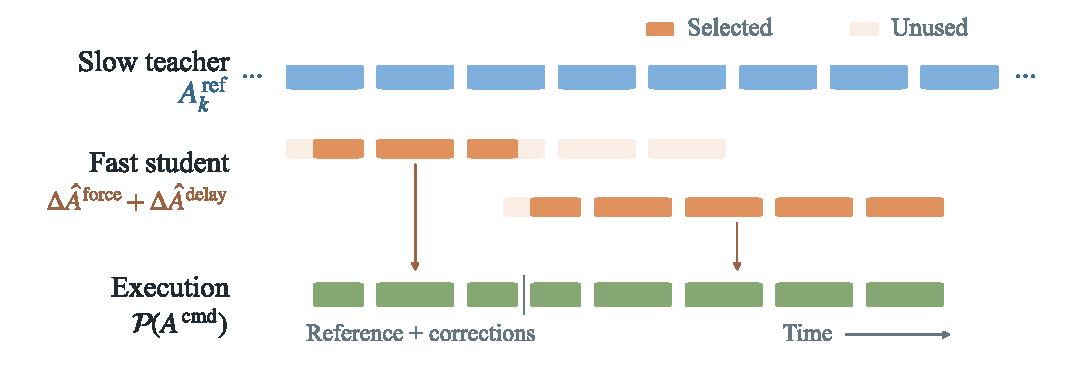
\includegraphics[width=0.82\textwidth]{figures/fig03_async_execution.pdf}
    \caption{Illustrative asynchronous execution with $K=5$. Correction queries read the latest completed base action at their start and retain it for command composition. A newly published correction chunk replaces the preceding chunk; numbered blocks show its active steps. Colors identify base-action updates, and dotted lines mark correction-query completion.}
    \label{fig:async_deployment}
\end{figure*}

Expired correction steps are skipped, and the remaining steps execute sequentially without interpolation. The base pose is interpolated by timestamp. The force and state-consistent delay corrections are bounded independently, added to the base action in normalized delta-action coordinates, and converted to an absolute command using the base-action query state. The supervised delay-correction target already includes $\Gamma(S_t,S_k)$.


\section{Experiments}
\label{sec:experiment}
\subsection{Experimental Setup}
\label{sec:exp_protocol}

\noindent\textbf{Hardware, tasks, and data collection.}
The evaluation includes $5$ single-arm and $4$ bimanual tasks on the two platforms shown in Fig.~\ref{fig:robot_setup}; the tasks are summarized in Fig.~\ref{fig:task_overview}. The single-arm platform is a 7-DoF Franka Emika Panda with wrist-mounted and external Intel RealSense D405 cameras. Demonstrations are collected using a 3Dconnexion SpaceMouse. The bimanual platform is an X Square Robot with one wrist-mounted camera per arm and one shared external camera. Demonstrations are collected through leader--follower teleoperation. Following ForceVLA~\cite{yu2025forcevlaenhancingvlamodels}, both platforms use robot-provided joint-torque-based wrench estimates without additional wrist force/torque sensors.

For each task, we collect $200$ demonstrations. Multi-view images, robot states, and commanded actions are recorded at $30$~Hz, and timestamped wrench estimates at $100$~Hz.

\begin{figure}[t]
    \centering
    \begin{minipage}[c]{0.45\columnwidth}
        \centering
        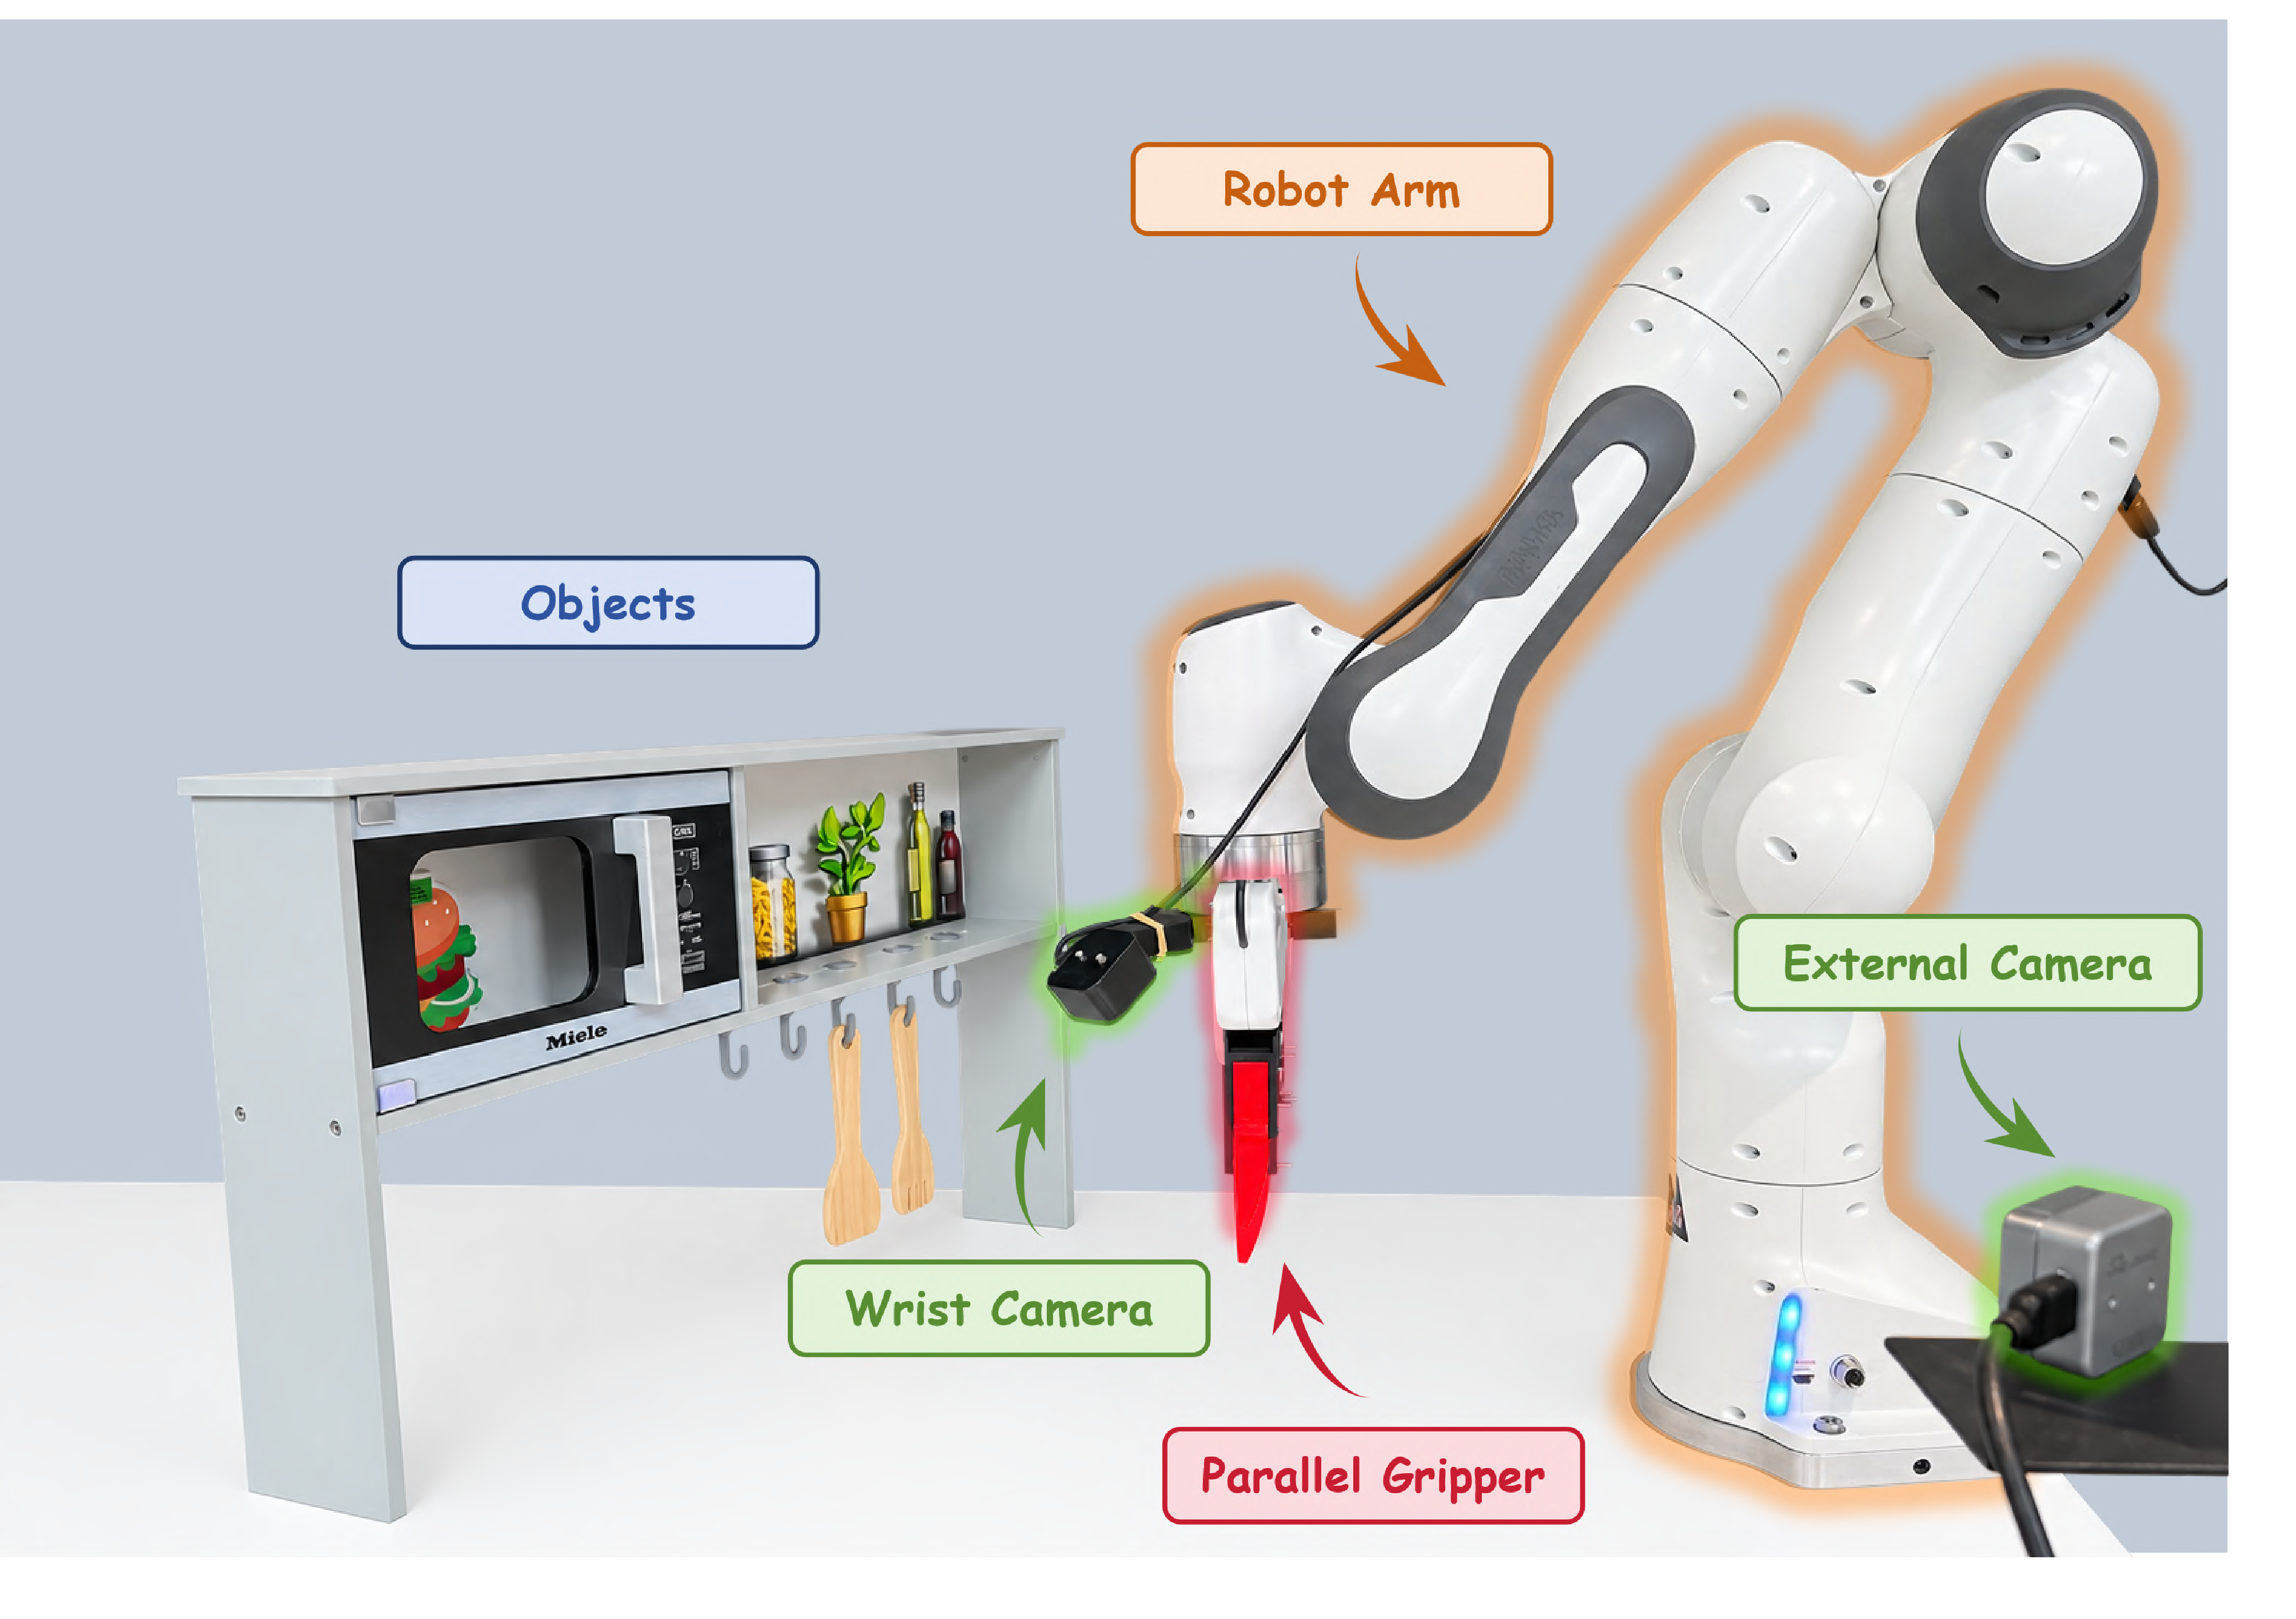
\includegraphics[width=\linewidth]{figures/fig04a_franka_platform.pdf}
    \end{minipage}\hspace{0.025\columnwidth}
    \begin{minipage}[c]{0.45\columnwidth}
        \centering
        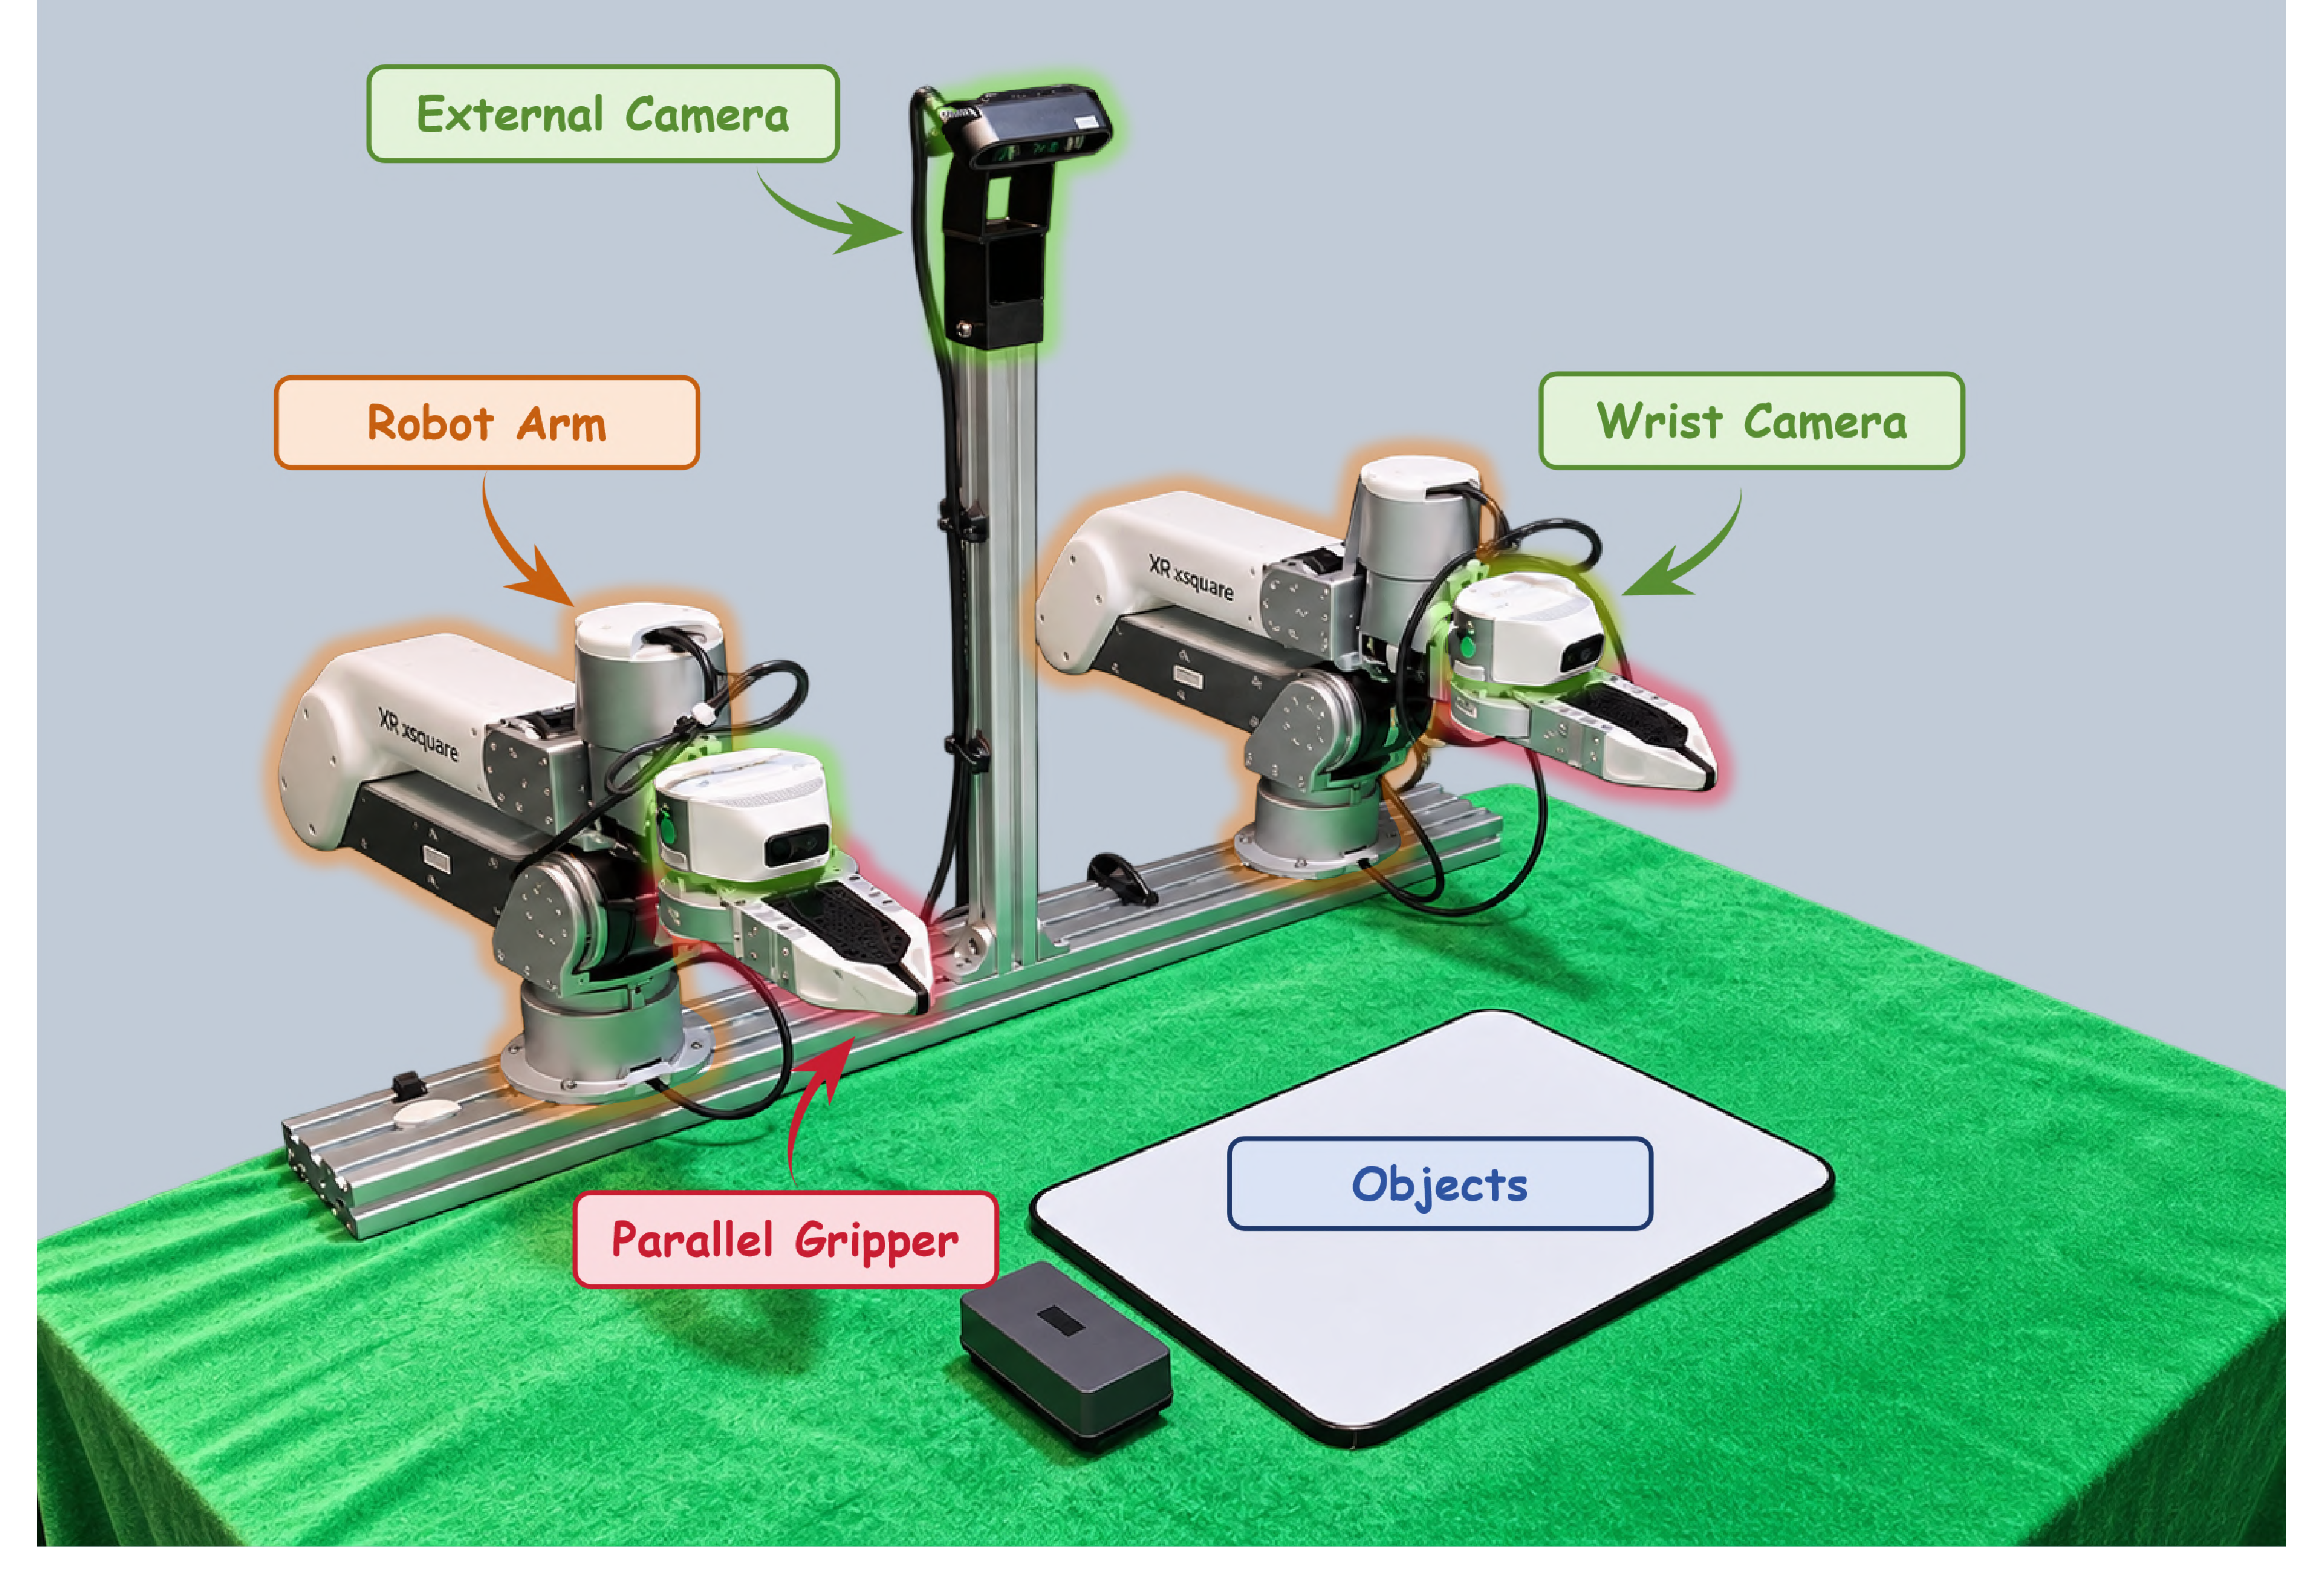
\includegraphics[width=\linewidth]{figures/fig04b_bimanual_platform.pdf}
    \end{minipage}
    \caption{Real-robot platforms. Left: single-arm Franka. Right: bimanual X Square Robot.}
    \label{fig:robot_setup}
\end{figure}

\begin{figure}[t]
    \centering
    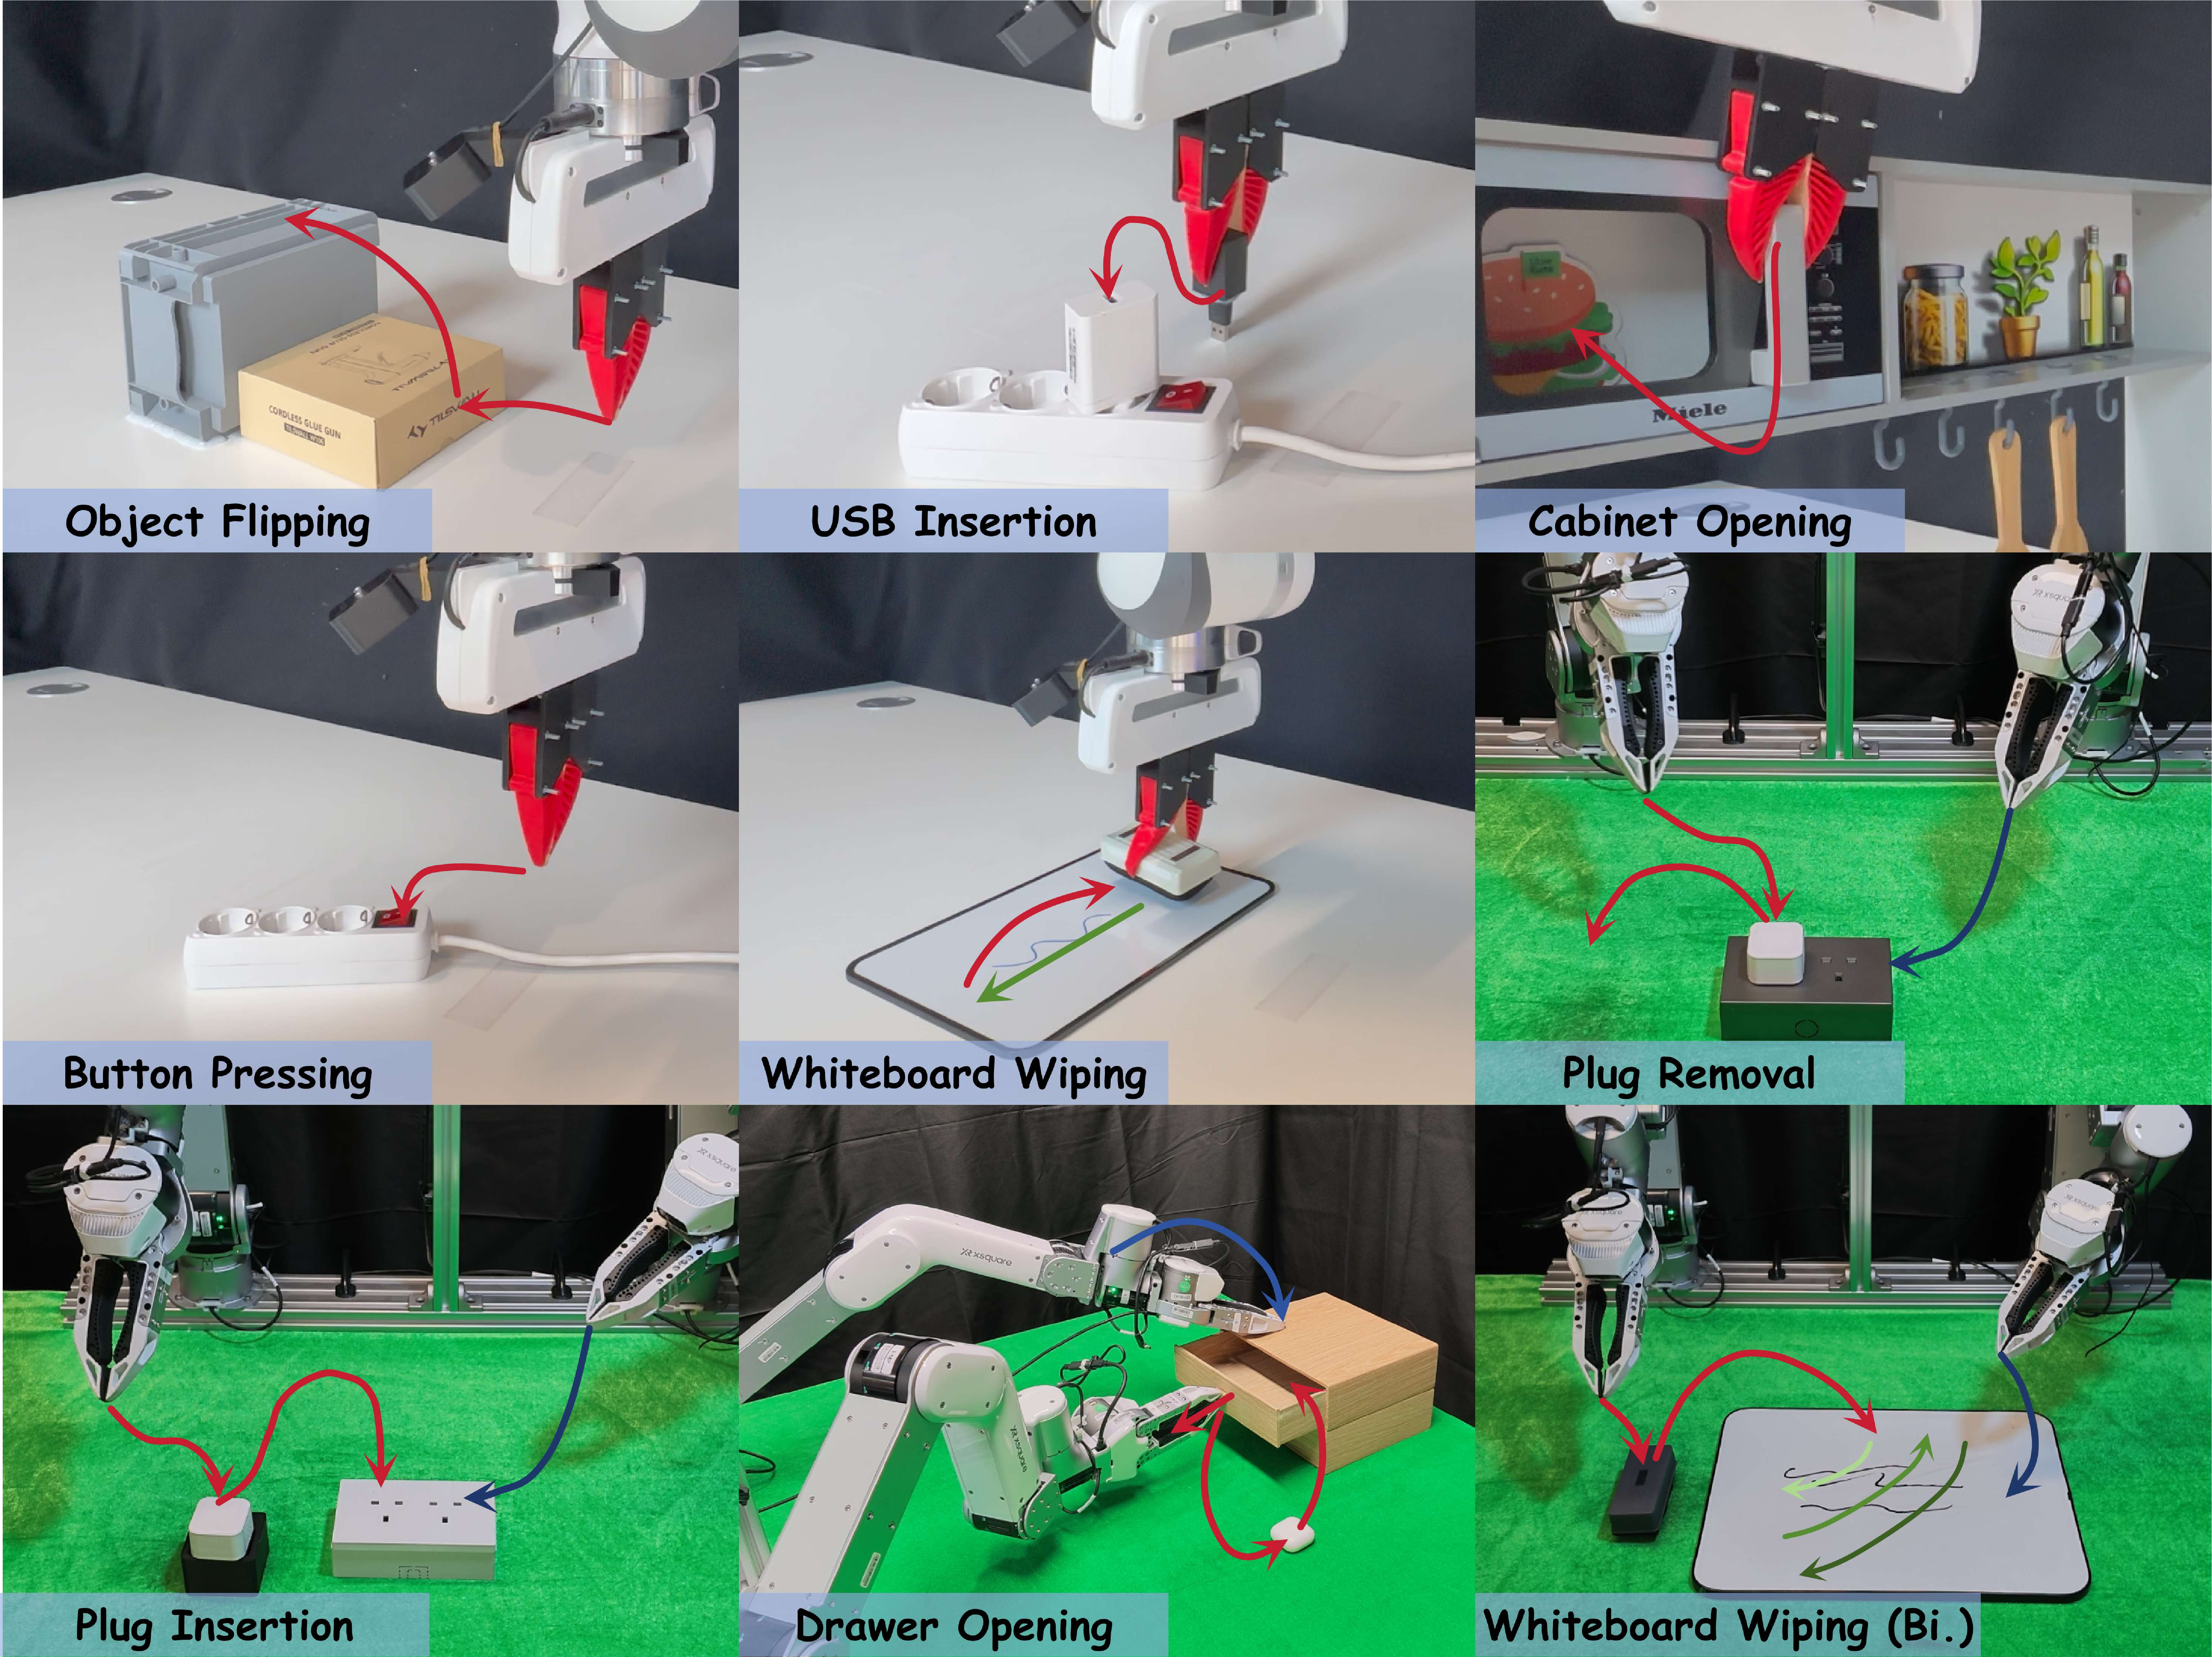
\includegraphics[width=\columnwidth]{figures/fig05_task_overview.pdf}
    \caption{The nine real-robot manipulation tasks used in the evaluation. The first five panels show single-arm tasks; the remaining four show bimanual tasks.}
    \label{fig:task_overview}
\end{figure}

\begin{table*}[!t]
    \centering
    \scriptsize
    \setlength{\tabcolsep}{3pt}
    \caption{Task success rate (\%) over 20 trials per method and task; Avg. is the mean across the nine tasks.}
    \label{tab:main_results}
    \begin{tabular}{lcccccccccc}
        \toprule
        & \multicolumn{5}{c}{\textbf{Single-arm}} & \multicolumn{4}{c}{\textbf{Bimanual}} & \\
        \cmidrule(lr){2-6}\cmidrule(lr){7-10}
        \textbf{Method}
        & \shortstack{Object\\Flipping}
        & \shortstack{USB\\Insertion}
        & \shortstack{Cabinet\\Opening}
        & \shortstack{Button\\Pressing}
        & \shortstack{Whiteboard\\Wiping}
        & \shortstack{Plug\\Removal}
        & \shortstack{Plug\\Insertion}
        & \shortstack{Drawer\\Opening}
        & \shortstack{Whiteboard\\Wiping}
        & \textbf{Avg.} \\
        \midrule
        $\pi_{0.5}$~\cite{intelligence2025pi05visionlanguageactionmodelopenworld} & 55.0 & 35.0 & 50.0 & 45.0 & 70.0 & 40.0 & 30.0 & 50.0 & 50.0 & 47.2 \\
        ForceVLA~\cite{yu2025forcevlaenhancingvlamodels} & 65.0 & 40.0 & 60.0 & 50.0 & 70.0 & 50.0 & 35.0 & 60.0 & 60.0 & 54.4 \\
        TA-VLA~\cite{zhang2025tavlaelucidatingdesignspace} & 65.0 & 35.0 & 60.0 & 60.0 & 75.0 & 55.0 & 40.0 & 60.0 & 65.0 & 57.2 \\
        ImplicitRDP~\cite{chen2026implicitrdpendtoendvisualforcediffusion} & 50.0 & 25.0 & 45.0 & 35.0 & 65.0 & 55.0 & 30.0 & 55.0 & 45.0 & 45.0 \\
        Temporal Teacher & 75.0 & 55.0 & 75.0 & 80.0 & 85.0 & 75.0 & 50.0 & 70.0 & 70.0 & 70.6 \\
        \textbf{ForceDelta-VLA (Ours)} & \textbf{90.0} & \textbf{80.0} & \textbf{80.0} & \textbf{85.0} & \textbf{90.0} & \textbf{80.0} & \textbf{70.0} & \textbf{80.0} & \textbf{85.0} & \textbf{82.2} \\
        \bottomrule
    \end{tabular}
\end{table*}

\noindent\textbf{Baselines and evaluation protocol.}
We compare with ForceVLA~\cite{yu2025forcevlaenhancingvlamodels}, a force-aware full-action policy that also provides our teacher backbone; $\pi_{0.5}$~\cite{intelligence2025pi05visionlanguageactionmodelopenworld}, a VLA without force/torque input; TA-VLA~\cite{zhang2025tavlaelucidatingdesignspace}, a torque-aware VLA; and ImplicitRDP~\cite{chen2026implicitrdpendtoendvisualforcediffusion}, a slow--fast visual--force policy. We also evaluate direct execution of the Stage-1 Temporal Teacher used by ForceDelta-VLA. All methods use the same task demonstrations, initial-state distributions, controller settings, and safety limits. We report success rate, peak contact force, and completion time.

\noindent\textbf{Implementation details.}
The teacher encodes a $100$-ms wrench history and predicts an action chunk with $H{=}50$ steps. The correction policy uses a causal force encoder and a shared attention module with separate force- and delay-correction heads to predict $K{=}5$ pose corrections. Deployment runs on a workstation with two NVIDIA RTX 4090 GPUs. The reference-action forward pass averages $189.7$~ms, corresponding to approximately $5$~Hz for serial inference (Table~\ref{tab:runtime}). Robot command transmission is limited to $100$~Hz; this control rate is distinct from the correction-query rate. Training and optimization details are provided in the supplementary material.

\subsection{Main Results}
\label{sec:exp_main}

\noindent\textbf{Quantitative results.}
Compared with the original ForceVLA baseline, the complete ForceDelta-VLA system improves mean success from $54.4\%$ to $82.2\%$ (Table~\ref{tab:main_results}). It also exceeds TA-VLA, $\pi_{0.5}$, and ImplicitRDP. Success improves over ForceVLA on all nine tasks, with the largest gains on USB Insertion, Button Pressing, and Plug Insertion.

Direct execution of the Stage-1 Temporal Teacher achieves $70.6\%$ mean success. ForceDelta-VLA improves mean success by about $11.7$ percentage points over this teacher. The largest gains are on USB Insertion and Plug Insertion, at $25$ and $20$ points, respectively. On Button Pressing, most of the improvement over ForceVLA is already obtained by the Temporal Teacher ($50\%$ to $80\%$); ForceDelta-VLA raises success to $85\%$.

\noindent\textbf{Contact force and completion time.}
Relative to ForceVLA, mean peak contact force over successful trials decreases by $4.2$~N on the single-arm platform and $4.3$~N on the bimanual platform, approximately $26\%$ on each (Table~\ref{tab:interaction}). Mean completion time decreases by $5.2$~s and $5.9$~s, respectively. Relative to the Temporal Teacher, the peak-force reductions are $3.3$~N and $2.2$~N, and completion time decreases by $3.9$~s and $3.4$~s.

\begin{table}[t]
    \centering
    \scriptsize
    \setlength{\tabcolsep}{2pt}
    \caption{Peak force and completion time, reported as mean $\pm$ standard deviation over successful trials pooled across tasks within each platform.}
    \label{tab:interaction}
    \begin{tabular}{lcccc}
        \toprule
        & \multicolumn{2}{c}{\textbf{Peak force} (N) $\downarrow$} & \multicolumn{2}{c}{\textbf{Completion time} (s) $\downarrow$} \\
        \cmidrule(lr){2-3}\cmidrule(lr){4-5}
        \textbf{Method} & Single & Biman. & Single & Biman. \\
        \midrule
        $\pi_{0.5}$ & $18.9 \pm 8.3$ & $20.4 \pm 9.1$ & $30.4 \pm 11.2$ & $33.1 \pm 12.8$ \\
        ForceVLA & $16.0 \pm 4.7$ & $16.8 \pm 6.2$ & $29.1 \pm 6.5$ & $31.7 \pm 9.4$ \\
        TA-VLA & $16.5 \pm 6.4$ & $15.9 \pm 4.8$ & $28.2 \pm 9.7$ & $30.0 \pm 7.1$ \\
        ImplicitRDP & $15.2 \pm 5.1$ & $14.8 \pm 4.9$ & $27.1 \pm 7.2$ & $27.4 \pm 7.8$ \\
        Temporal Teacher & $15.1 \pm 5.8$ & $14.7 \pm 4.3$ & $27.8 \pm 8.8$ & $29.2 \pm 6.9$ \\
        \textbf{\shortstack[l]{ForceDelta-VLA\\(Ours)}} & $\mathbf{11.8} \pm 3.4$ & $\mathbf{12.5} \pm 2.9$ & $\mathbf{23.9} \pm 5.4$ & $\mathbf{25.8} \pm 7.6$ \\
        \bottomrule
    \end{tabular}
\end{table}

\noindent\textbf{Qualitative results.}
Figure~\ref{fig:qualitative_button} highlights how the learned translational correction evolves through contact. The correction is smaller before sustained contact, increases during pressing, shows a brief change near peak contact, and decreases as contact is released.

\begin{figure}[t]
    \centering
    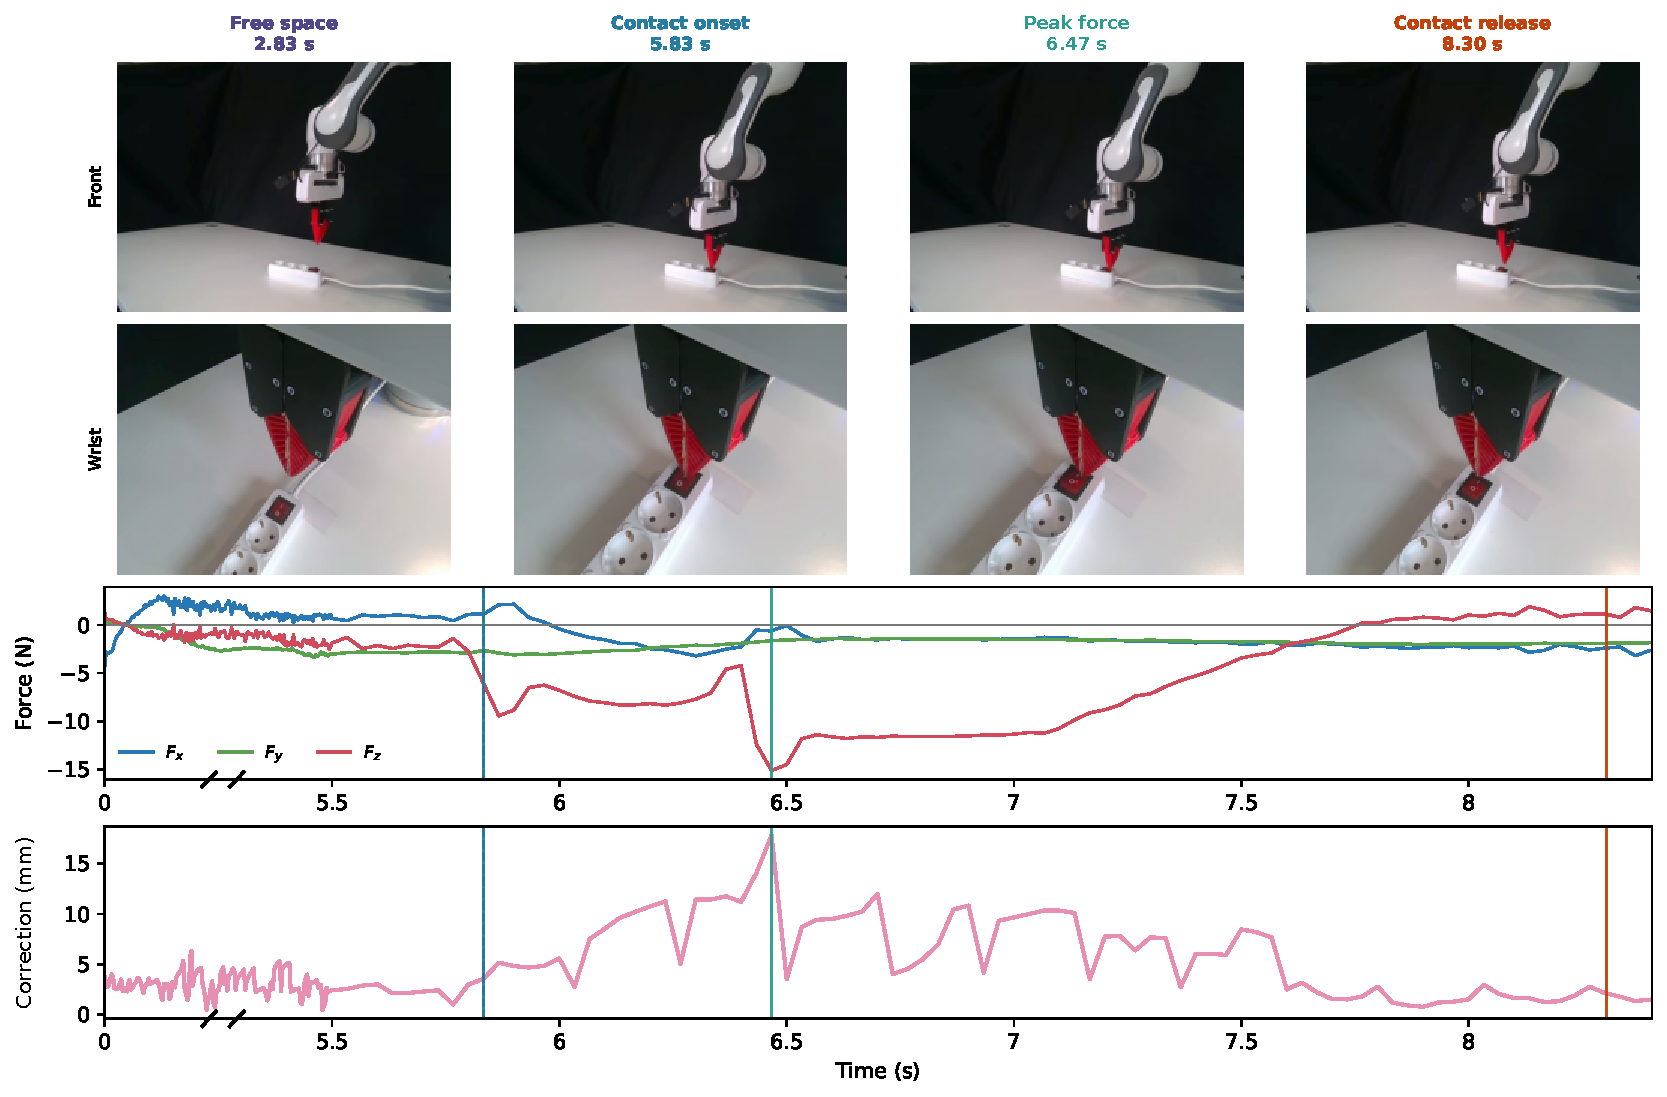
\includegraphics[width=\columnwidth]{figures/fig06_button_pressing_rollout.pdf}
    \caption{Representative rollout of Button Pressing. The observations show four interaction phases. The traces plot robot-estimated end-effector force components and translational correction magnitude over the contact interval; vertical lines mark the three displayed contact transitions, while the earlier free-space frame precedes the axis break.}
    \label{fig:qualitative_button}
\end{figure}

\subsection{Runtime and Reference-Action Delay}
\label{sec:exp_runtime}

We measure the forward-pass latencies of the reference-action and correction pathways and evaluate task performance under additional reference-action latency.

\noindent\textbf{Forward-pass latency.}
The correction forward pass takes $2.43$~ms, below the $10$-ms interval between robot command transmissions (Table~\ref{tab:runtime}). The Temporal Teacher and reference-action forward passes both exceed that interval. By reusing a reference action, the correction pathway avoids a new generative prediction at each query.

\begin{table}[t]
    \centering
    \scriptsize
    \setlength{\tabcolsep}{2pt}
    \caption{Forward-pass latency with batch size one under the Button Pressing deployment workload, reported as mean $\pm$ standard deviation over repeated passes on the deployment workstation.}
    \label{tab:runtime}
    \begin{tabular}{lc}
        \toprule
        \textbf{Method/path} & \textbf{Forward latency (ms)} $\downarrow$ \\
        \midrule
        ImplicitRDP & $12.86 \pm 0.23$ \\
        Temporal Teacher & $176.4 \pm 5.9$ \\
        ForceDelta reference action & $189.7 \pm 6.8$ \\
        ForceDelta correction & $\mathbf{2.43} \pm 0.12$ \\
        \bottomrule
    \end{tabular}
\end{table}

\noindent\textbf{Sensitivity to reference-action delay.}
We evaluate USB Insertion and Plug Insertion with $0$, $100$, and $200$~ms of additional reference-action latency, using $10$ trials per task, method, and delay. From $0$ to $200$~ms of additional delay, success decreases by $15$ percentage points for ForceDelta-VLA and $25$ points for the Temporal Teacher (Fig.~\ref{fig:latency_sensitivity}). Mean peak force over successful trials increases by $3.7$~N and $9.6$~N, respectively. These results support updating corrections between reference-action updates.

\begin{figure}[t]
    \centering
    \begin{minipage}[c]{0.49\columnwidth}
        \centering
        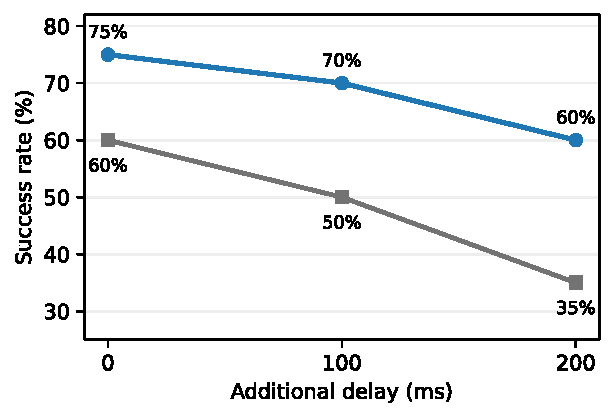
\includegraphics[width=\linewidth]{figures/fig07a_delay_success.pdf}
    \end{minipage}\hfill
    \begin{minipage}[c]{0.49\columnwidth}
        \centering
        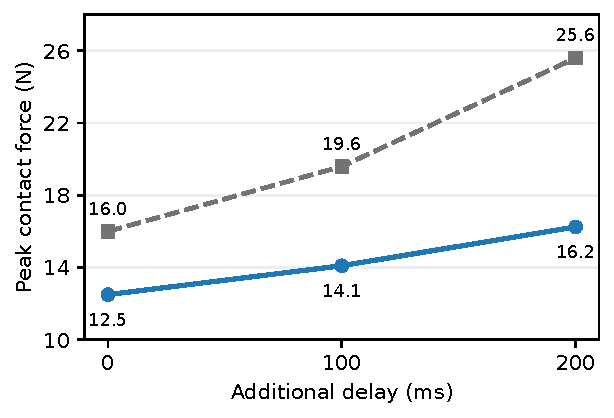
\includegraphics[width=\linewidth]{figures/fig07b_delay_peak_force.pdf}
    \end{minipage}
    \caption{Sensitivity to additional reference-action latency on the two insertion tasks. Left: success rate. Right: peak force over successful trials. Blue solid lines with circular markers denote ForceDelta-VLA; gray dashed lines with square markers denote Temporal Teacher.}
    \label{fig:latency_sensitivity}
\end{figure}

\subsection{Ablation Studies}
\label{sec:exp_ablation}

The ablations ask three questions: how the correction target should be defined, whether the fast policy should predict separate corrections, a combined correction, or complete actions, and how training should account for asynchronous execution (Table~\ref{tab:ablation}). All variants are evaluated on USB Insertion, single-arm Whiteboard Wiping, Plug Insertion, and Drawer Opening.

\noindent\textbf{Ablation setup.}
Execution ablations retain the trained model: \textbf{Reference action only} disables both corrections; \textbf{w/o force correction} disables the force output; \textbf{w/o learned delay correction} disables the full delay output, including reference-state alignment; and \textbf{Zeroed correction input} supplies an all-zero force history while retaining the force branch. The remaining variants retrain the affected policy. Their changes are described with the corresponding results below.

\begin{table}[t]
    \centering
    \scriptsize
    \setlength{\tabcolsep}{2pt}
    \caption{Ablations on four tasks, with 20 trials per task. Peak force: mean $\pm$ standard deviation over successful trials.}
    \label{tab:ablation}
    \begin{tabular}{lcccc}
        \toprule
        & \multicolumn{2}{c}{\textbf{Success rate} (\%) $\uparrow$}
        & \multicolumn{2}{c}{\textbf{Peak force} (N) $\downarrow$} \\
        \cmidrule(lr){2-3}\cmidrule(lr){4-5}
        \textbf{Variant} & \textbf{Single} & \textbf{Biman.}
        & \textbf{Single} & \textbf{Biman.} \\
        \midrule
        \multicolumn{5}{l}{\emph{Execution/component ablations}} \\
        Reference action only & $62.5$ & $50.0$ & $16.7 \pm 6.9$ & $18.2 \pm 7.6$ \\
        w/o force correction & $70.0$ & $57.5$ & $15.4 \pm 5.8$ & $17.1 \pm 6.3$ \\
        \shortstack[l]{w/o learned\\delay correction} & $77.5$ & $67.5$ & $13.2 \pm 4.1$ & $14.5 \pm 5.0$ \\
        Zeroed correction input & $65.0$ & $55.0$ & $15.9 \pm 6.4$ & $17.7 \pm 7.0$ \\
        \textbf{ForceDelta-VLA (full)} & $\mathbf{85.0}$ & $\mathbf{75.0}$ & $\mathbf{11.7} \pm 3.1$ & $\mathbf{12.8} \pm 3.8$ \\
        \midrule
        \multicolumn{5}{l}{\emph{Supervision/decomposition ablations}} \\
        \shortstack[l]{Demonstration-derived\\correction target} & $72.5$ & $57.5$ & $14.6 \pm 5.2$ & $16.5 \pm 6.1$ \\
        \shortstack[l]{Zero-wrench\\teacher query} & $65.0$ & $55.0$ & $16.1 \pm 6.7$ & $17.3 \pm 6.5$ \\
        w/o schedule replay & $77.5$ & $62.5$ & $13.8 \pm 4.7$ & $15.6 \pm 5.8$ \\
        \shortstack[l]{Single combined-\\correction head} & $75.0$ & $65.0$ & $13.5 \pm 4.3$ & $14.9 \pm 4.9$ \\
        \shortstack[l]{Fast full-action\\distillation} & $67.5$ & $52.5$ & $15.2 \pm 5.6$ & $17.9 \pm 7.4$ \\
        \textbf{ForceDelta-VLA (full)} & $\mathbf{85.0}$ & $\mathbf{75.0}$ & $\mathbf{11.7} \pm 3.1$ & $\mathbf{12.8} \pm 3.8$ \\
        \bottomrule
    \end{tabular}
\end{table}

\begin{samepage}
\noindent\textbf{How should correction supervision be defined?}
\textbf{Demonstration-derived correction target} replaces the force target with the demonstrated action minus the force-agnostic teacher prediction at the same query state. Success decreases by $12.5$ and $17.5$ percentage points on the single-arm and bimanual platforms, respectively. This comparison favors defining force supervision through teacher predictions matched in context, state, and sampling noise. \textbf{Zero-wrench teacher query}, used for both reference generation and target construction, also lowers success, supporting the learned force-agnostic mode.

\end{samepage}

\noindent\textbf{What should the fast policy predict?}
Removing the force correction reduces success by $15$ and $17.5$ percentage points and increases mean peak force over successful trials by $3.7$ and $4.3$~N on the single-arm and bimanual platforms, respectively. The force branch thus contributes to both task completion and contact-force reduction. Removing both corrections lowers success further. Zeroing the force history also performs worse than disabling the force output, indicating that the active branch depends on force feedback.

\textbf{Single combined-correction head} trains one head on the summed target and reduces success by $10$ percentage points on both platforms, favoring separate supervision and prediction of the two corrections. \textbf{Fast full-action distillation} of the teacher's pose actions also performs worse under the same compact student architecture, inputs, and update schedule. This favors reusing reference actions and assigning the student to predict their corrections.

\noindent\textbf{How does asynchronous adaptation contribute?}
Disabling the learned delay correction reduces success by $7.5$ percentage points on both platforms and increases peak force, supporting the adjustment for reference-action mismatch and reference-state alignment. Omitting \textbf{schedule replay} reduces success by $7.5$ and $12.5$ percentage points on the single-arm and bimanual platforms, respectively. The student therefore also benefits from training on delayed references.

\subsection{Generalization to Unseen Objects}
\label{sec:exp_physical_generalization}

We evaluate USB Insertion, Object Flipping, and bimanual Whiteboard Wiping with the unseen objects shown in Fig.~\ref{fig:physical_generalization_objects}.

\begin{table}[!htbp]
    \centering
    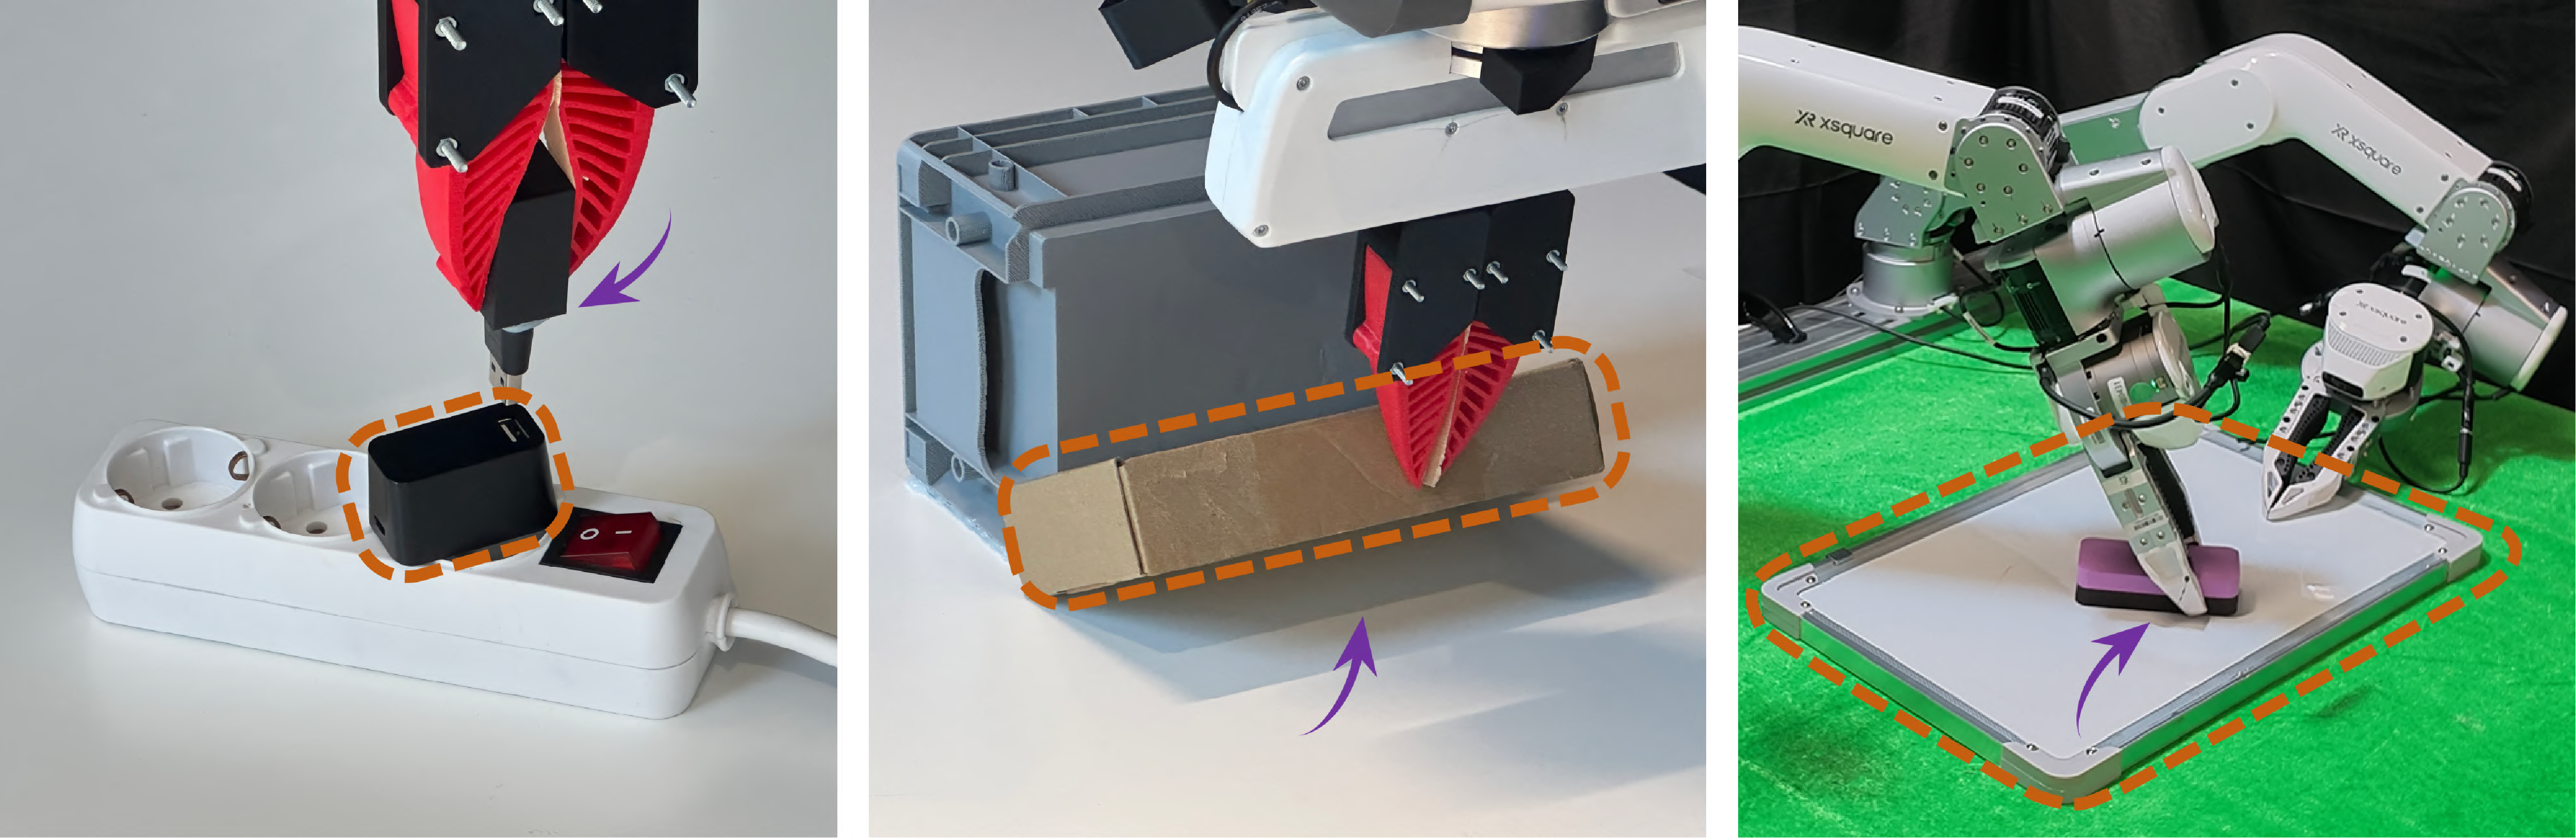
\includegraphics[width=0.85\columnwidth]{figures/fig08_unseen_objects.pdf}
    \begingroup
    \captionof{figure}{Generalization evaluation. From left to right: USB Insertion, Object Flipping, and bimanual Whiteboard Wiping.}
    \label{fig:physical_generalization_objects}
    \endgroup

    \scriptsize
    \setlength{\tabcolsep}{5pt}
    \caption{Generalization with unseen objects: 10 trials per task, 30 per method. Peak force: mean $\pm$ standard deviation over successful trials.}
    \label{tab:physical_generalization}
    \begin{tabular}{lcc}
        \toprule
        \textbf{Method} & \textbf{Success rate} (\%) $\uparrow$ & \textbf{Peak force} (N) $\downarrow$ \\
        \midrule
        ImplicitRDP & $16.7$ & $45.9 \pm 10.5$ \\
        Temporal Teacher & $40.0$ & $21.8 \pm 5.2$ \\
        \textbf{ForceDelta-VLA (Ours)} & $66.7$ & $13.6 \pm 3.7$ \\
        \bottomrule
    \end{tabular}
\end{table}

On unseen objects, ForceDelta-VLA improves success over the Temporal Teacher by $26.7$ percentage points and reduces mean peak force over successful trials by $8.2$~N (Table~\ref{tab:physical_generalization}). The new USB port is particularly challenging for the Temporal Teacher. For ImplicitRDP, failures often occur while establishing contact: the policy misses the replacement eraser during grasping or fails to initiate the downward insertion motion.

\subsection{Failure Analysis}
\label{sec:exp_limitations}

In failed USB and plug insertion trials, the robot often reached the target region but contacted the rim or entered with a small orientation error. Once the connector jammed, the reference action often continued advancing, and the corrected motion did not retreat far enough to clear the jam and retry.

In cabinet and drawer opening, pulling sometimes began before stable contact with the handle was established. Recovery required releasing contact, repositioning the gripper, or approaching again. Wiping and object-flipping failures involved contact on an unintended side or loss of the intended contact geometry, requiring a different approach direction.

Reference-update delay further reduced insertion success (Fig.~\ref{fig:latency_sensitivity}). During this delay, the robot could enter a new contact state while the student continued correcting a chunk generated before that change. These failures point to the need for reference updates that initiate retreat, reestablish contact, or change the approach direction.

\FloatBarrier

\section{Conclusion and Future Work}
\label{sec:conclusion}
We presented ForceDelta-VLA, a correction-distillation framework for contact-rich manipulation. Paired force-conditioned and force-agnostic teacher predictions define force-correction targets, while delay-correction targets account for reference-action mismatch and reference-state alignment. The correction policy is trained with asynchronous schedule replay and updates pose corrections between reference-action updates. Across nine real-robot tasks, ForceDelta-VLA achieved $82.2\%$ mean success, compared with $54.4\%$ for ForceVLA and $70.6\%$ for direct execution of the Stage-1 Temporal Teacher. Mean successful-trial peak contact force was approximately $26\%$ lower than that of ForceVLA on both platforms.

Future work will study when to refresh reference actions and how to recover when the required motion exceeds the correction bounds.

\vspace{0.1in}
% \noindent\textbf{Acknowledgement}

{
\small
\bibliographystyle{IEEEtran}
\bibliography{main}
}


\end{document}
